\documentclass[12pt]{article}
\usepackage{graphicx}
\usepackage{fancyhdr}
\usepackage{hyperref}

\title{Chapter 3: Processes}
\author{Muhammad Shafeen \\ 22P-9278 }
\date{}

\begin{document}
\maketitle
\tableofcontents

\section{3.1.1 Exercise}

Write a code that finds the following:
\begin{itemize}
    \item PID value for \texttt{myfirst.c}
    \item PPID value for \texttt{myfirst.c}
    \item Process name from the PPID value (using \texttt{pstree -p | grep <PPID>}).
\end{itemize}

\subsection{Screenshot of Exercise Code 1}
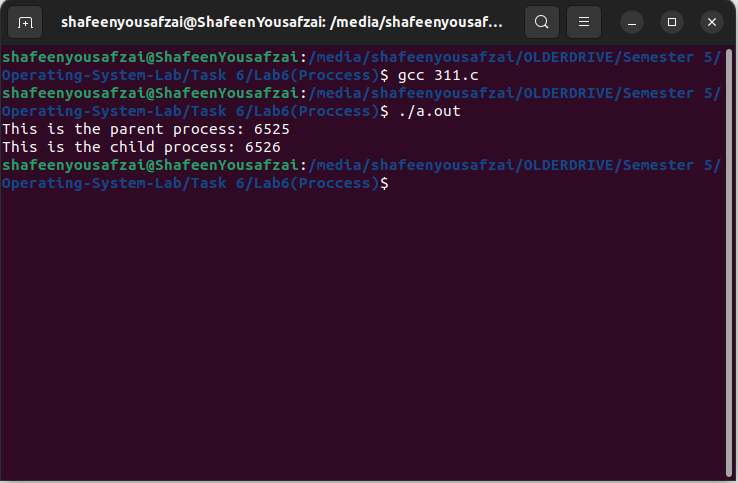
\includegraphics[width=\textwidth]{image.png} % Insert screenshot here

\subsection{Tree of Code 1}
    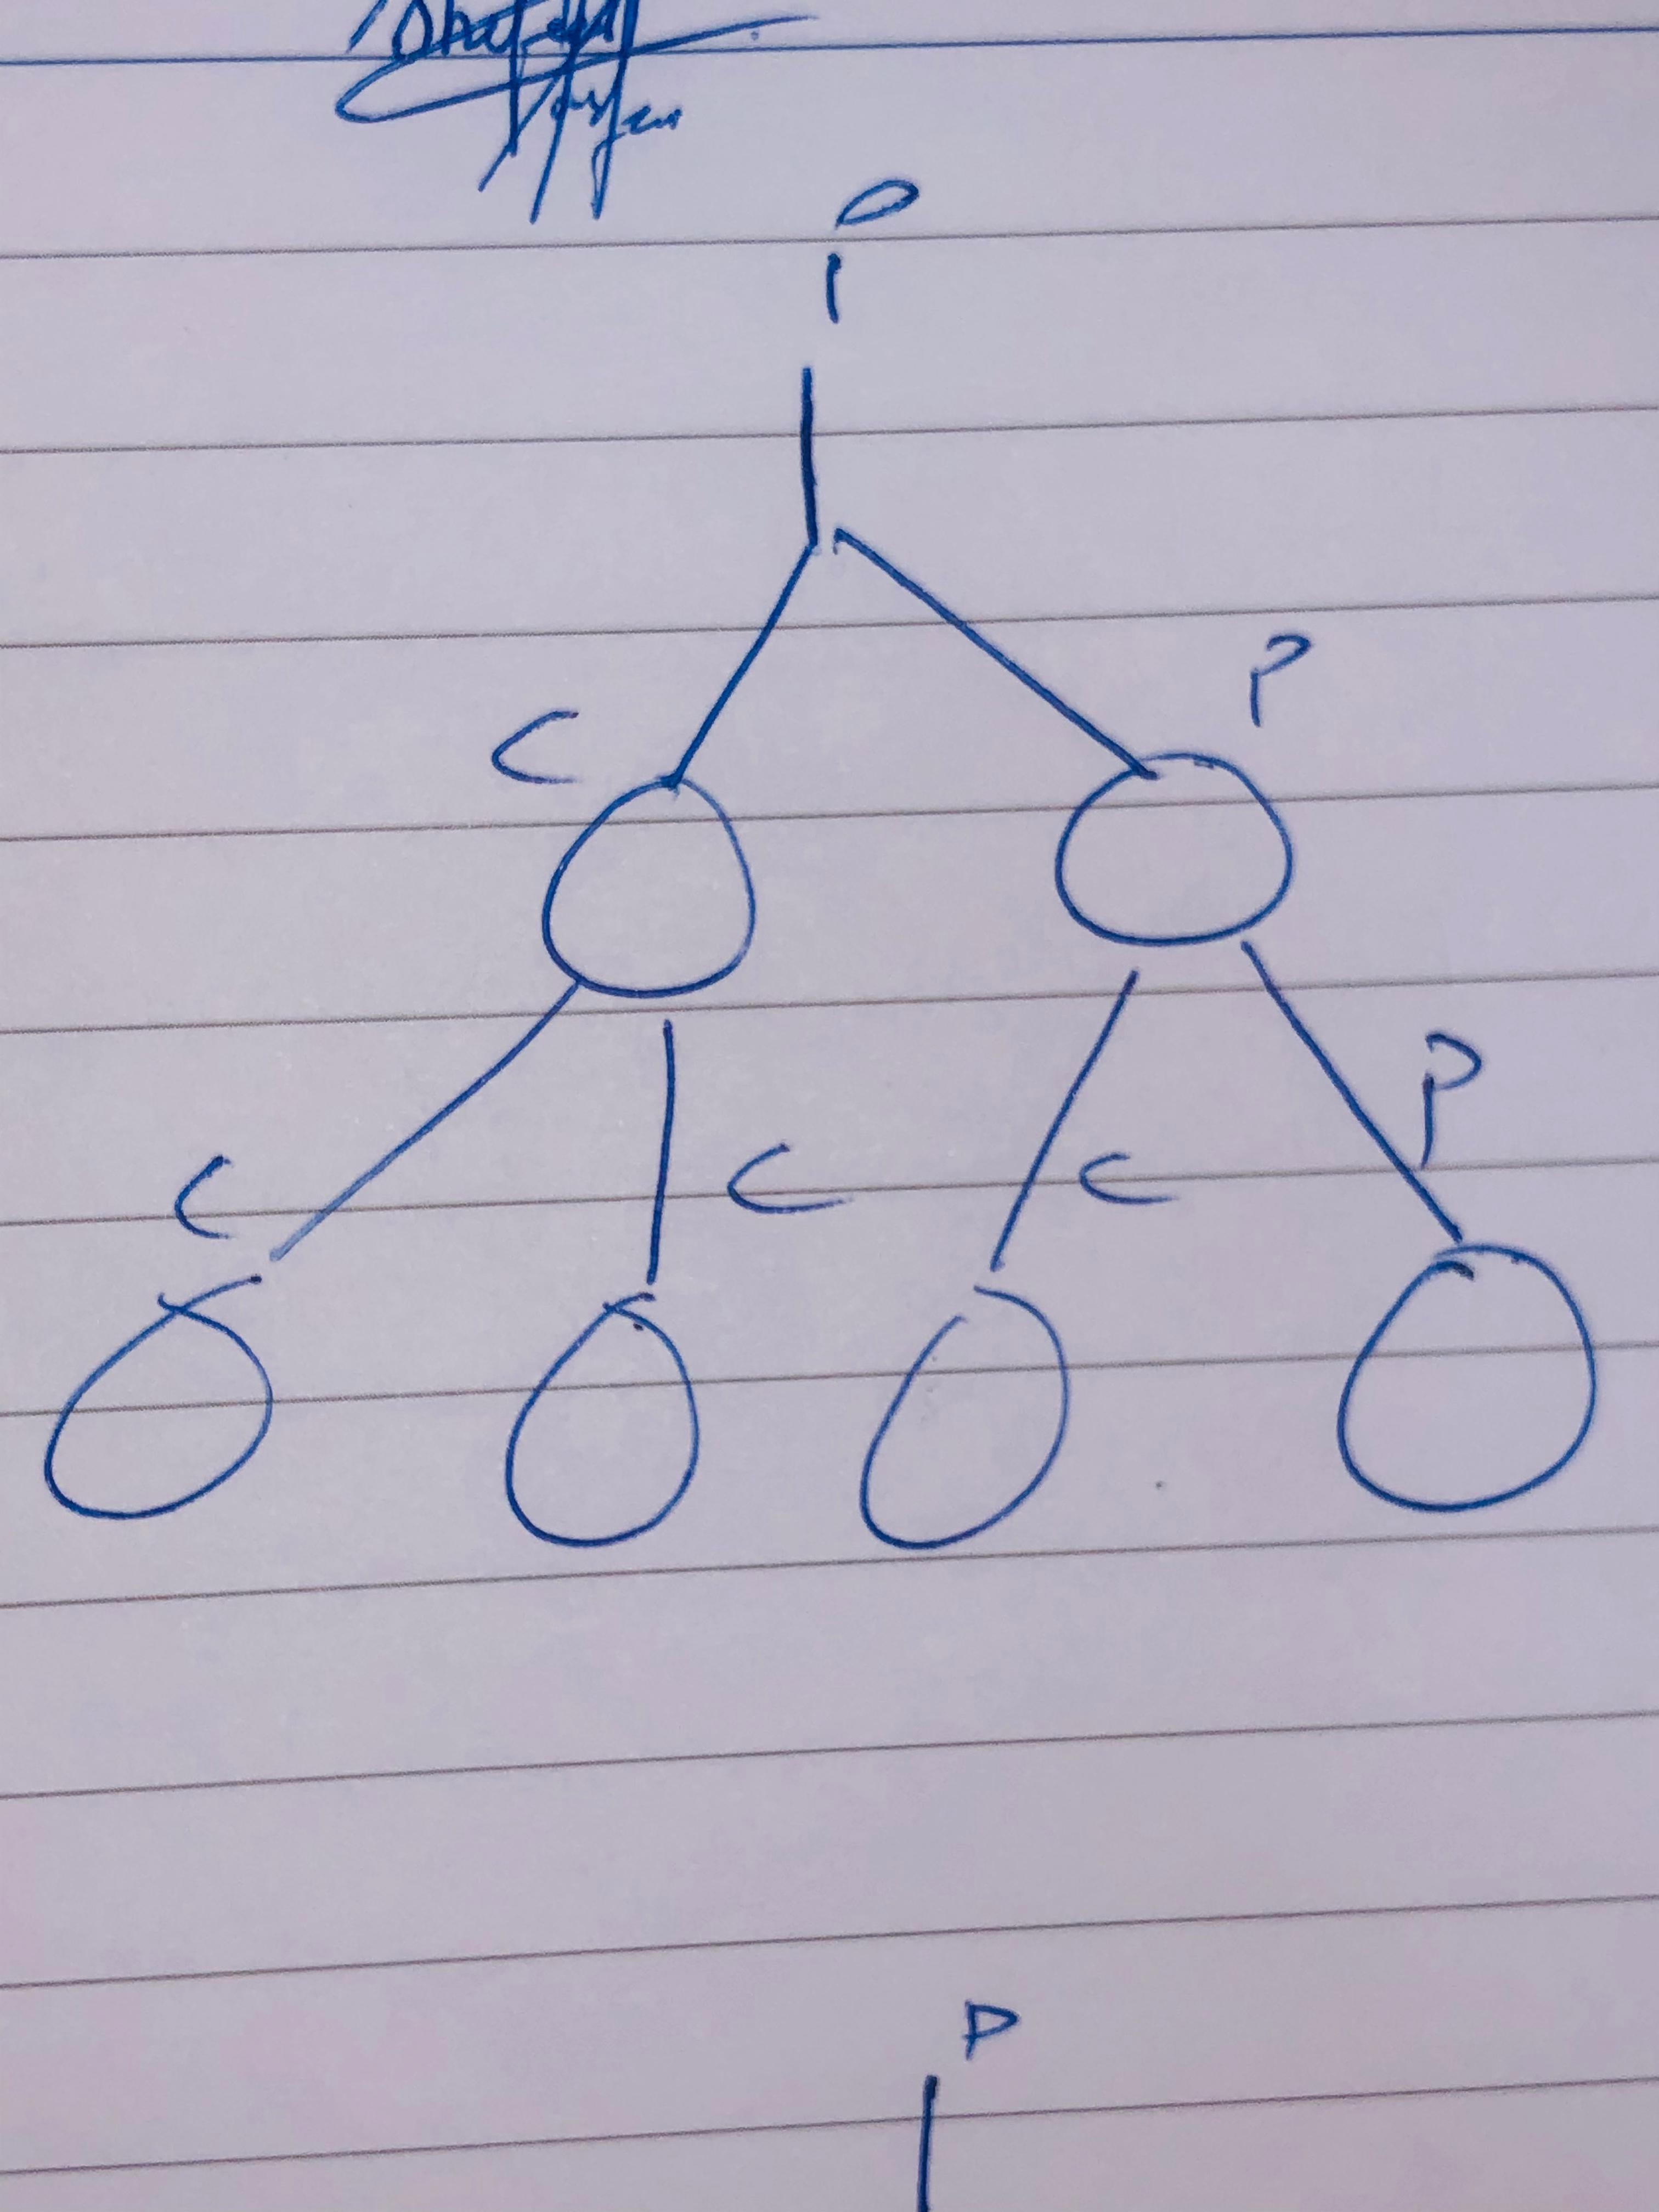
\includegraphics[width=\textwidth]{Untitled.jpeg}


\subsection{Screenshot of Exercise Code 2}
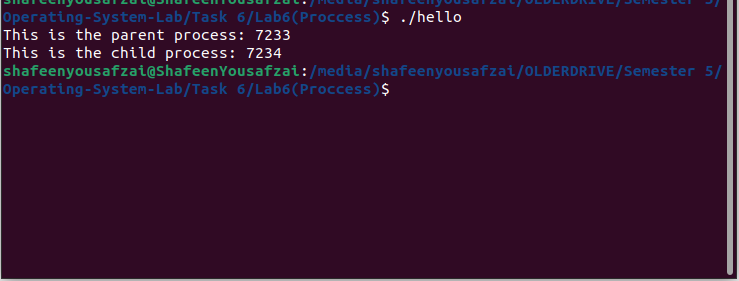
\includegraphics[width=\textwidth]{Screenshot from 2024-09-27 05-33-32.png} % Insert screenshot here

\subsection{Tree of Code 2}
    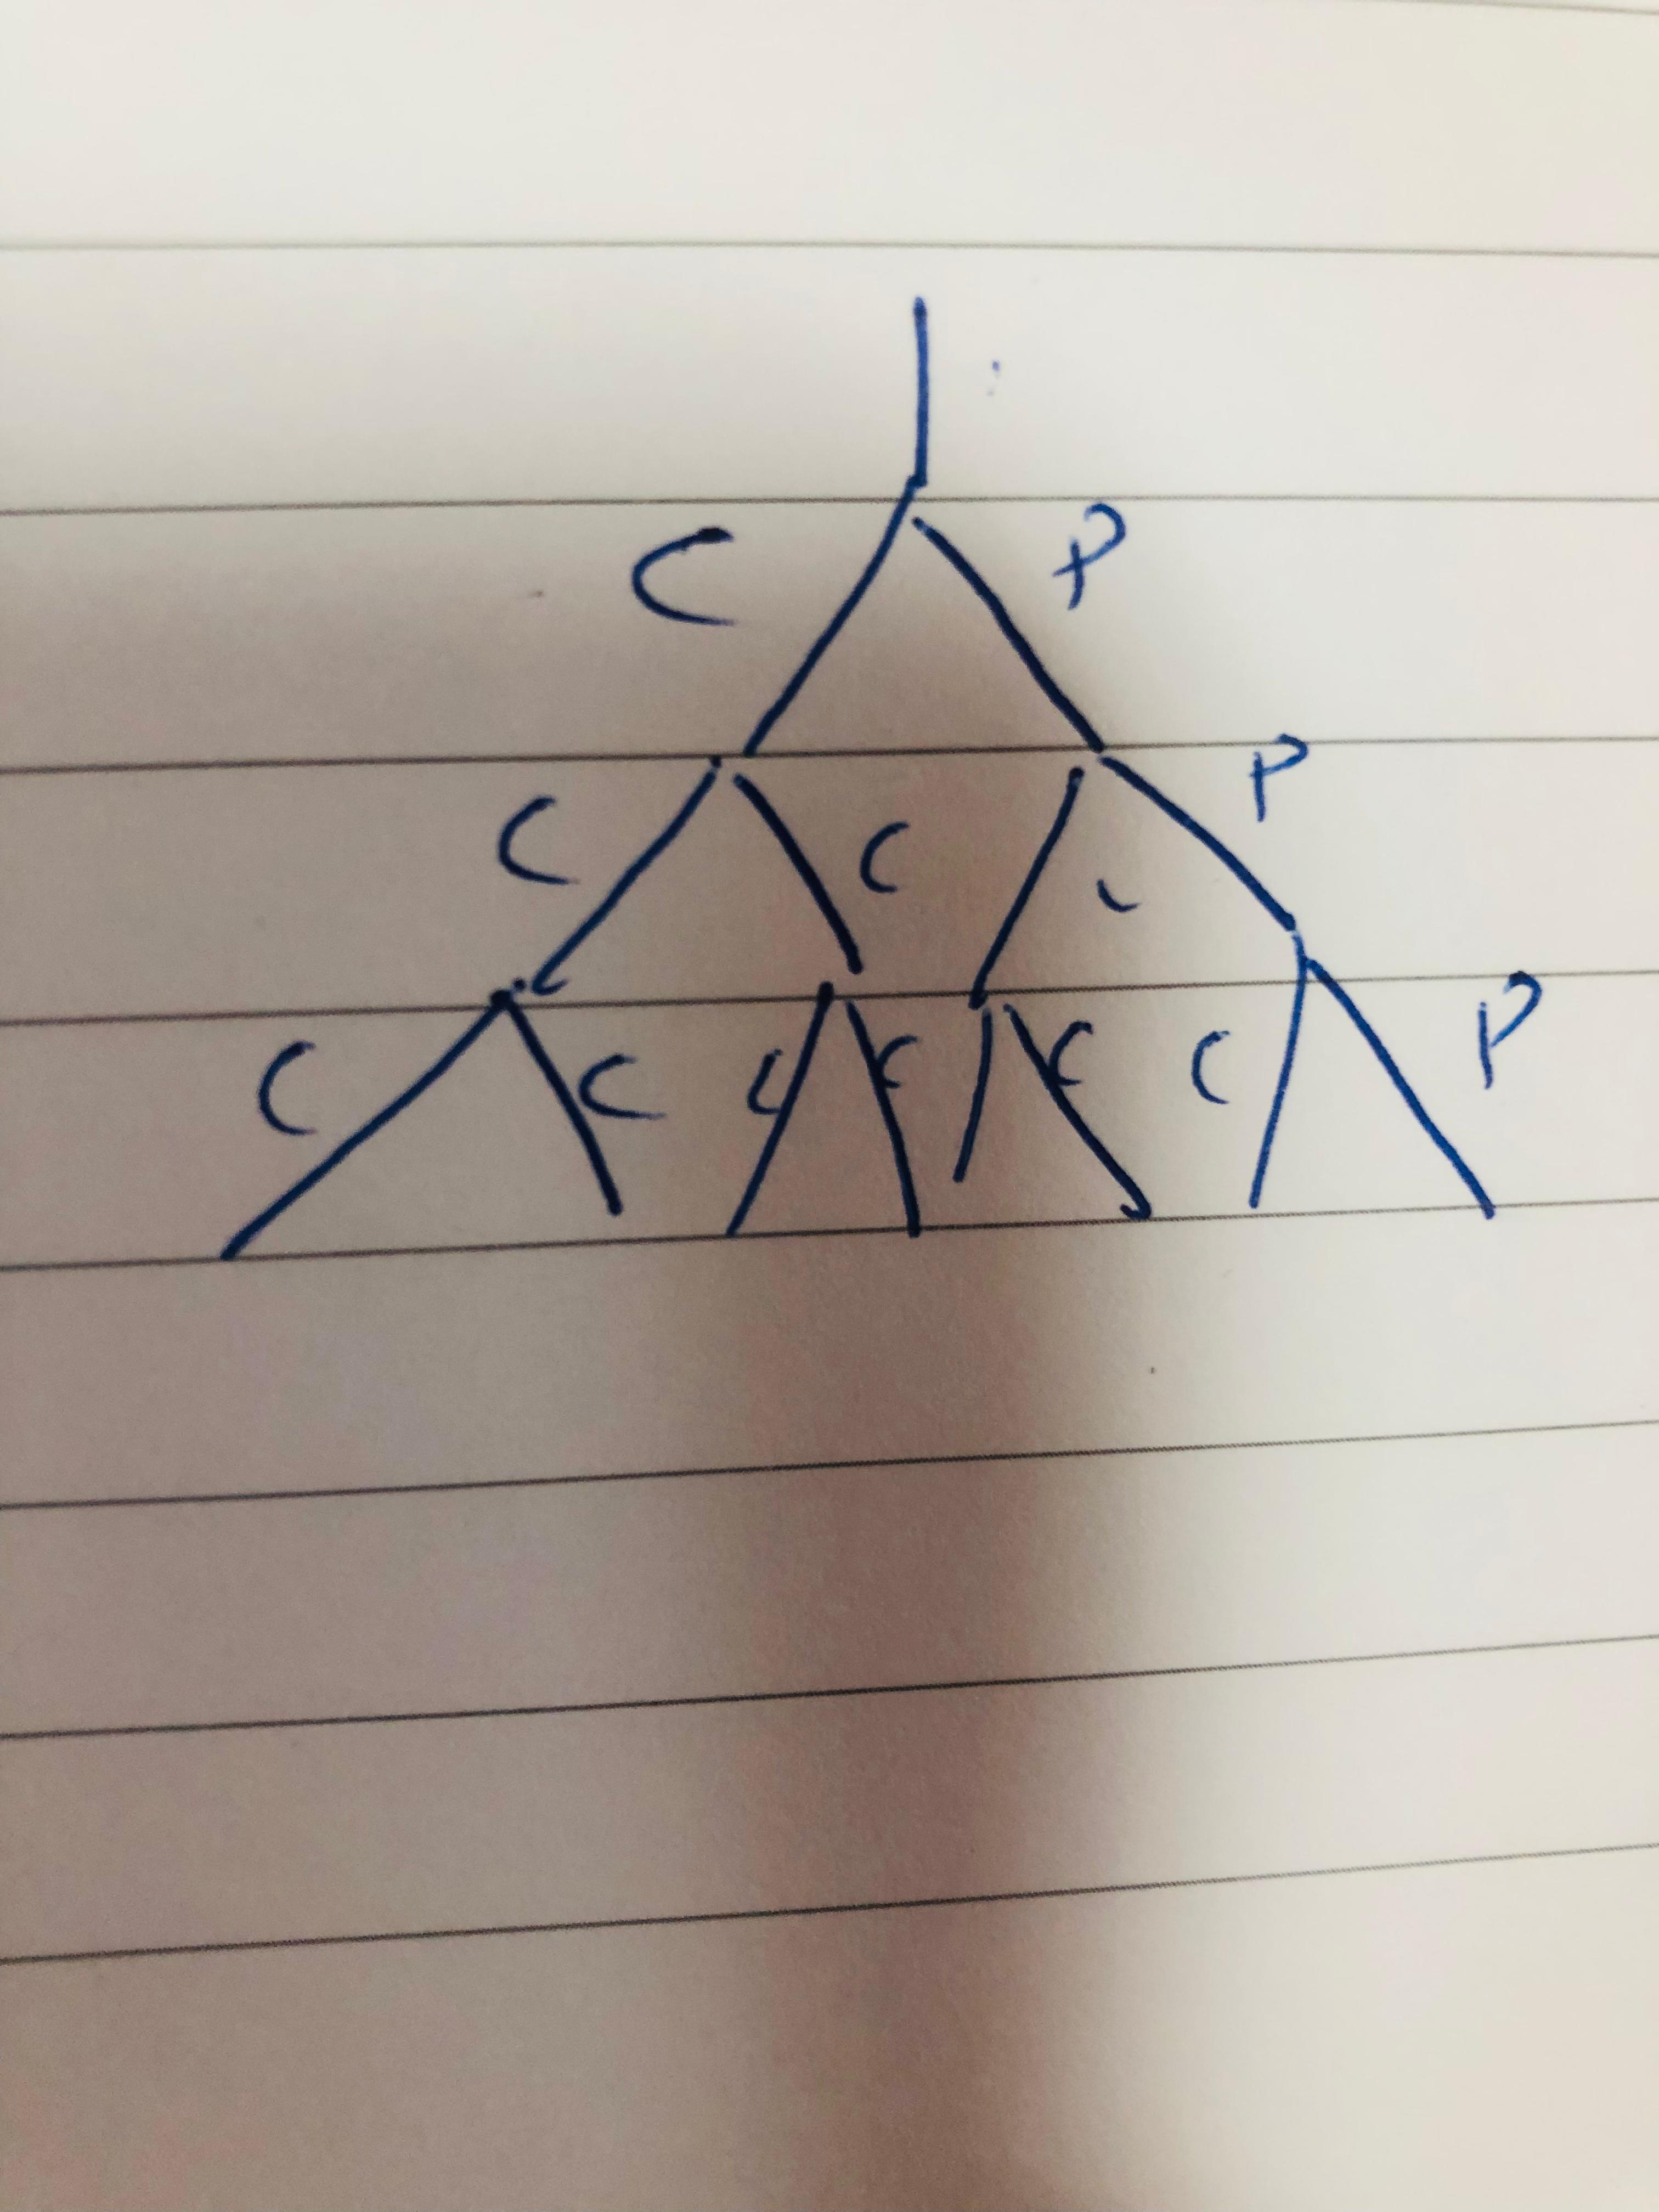
\includegraphics[width=\textwidth]{Untitled1.jpeg}



\subsection{Q1 Answer}
  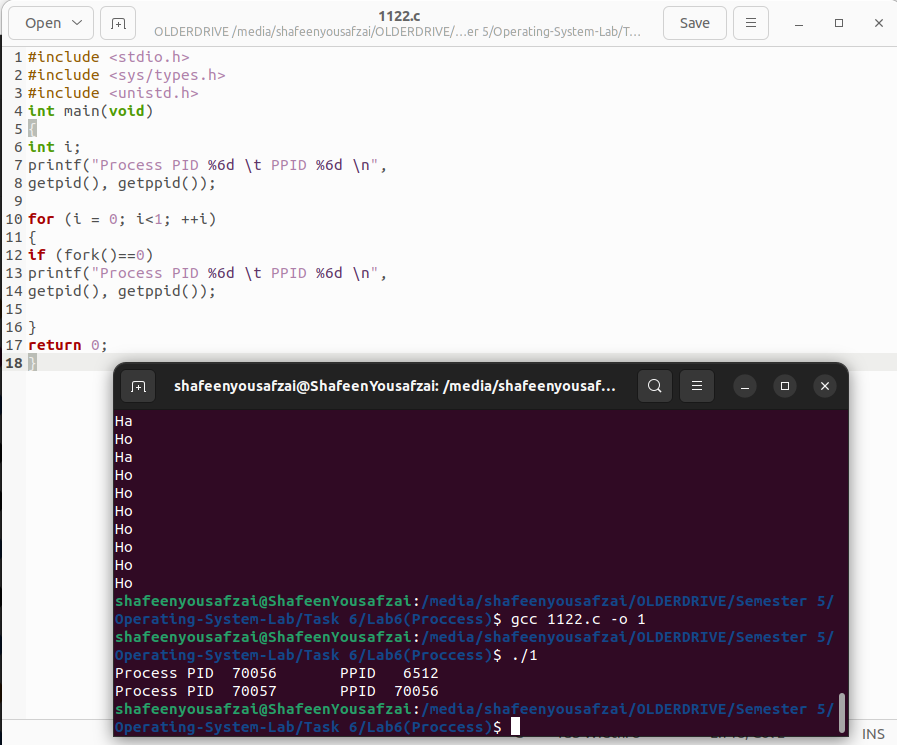
\includegraphics[width=\textwidth]{Screenshot from 2024-09-27 05-46-26.png}   

\subsection{loop from i<1 to i<2}
 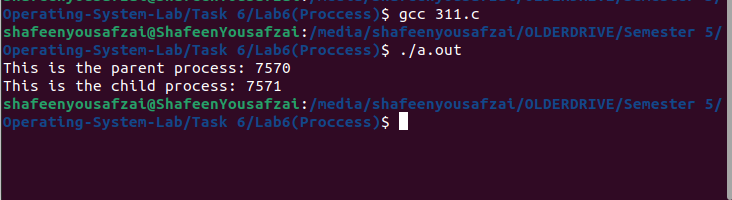
\includegraphics[width=\textwidth]{Screenshot from 2024-09-27 05-37-44.png}
\subsection{to i<3}
 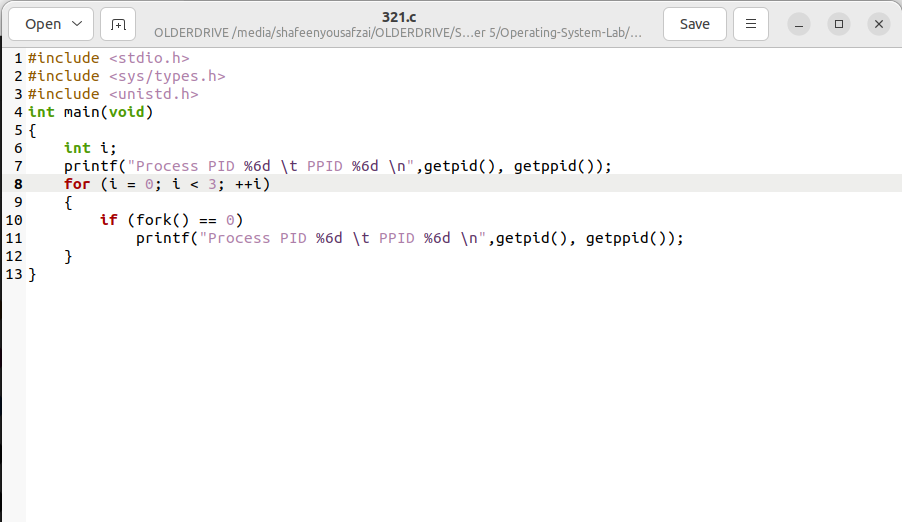
\includegraphics[width=\textwidth]{Screenshot from 2024-09-27 05-37-58.png}
    \\
  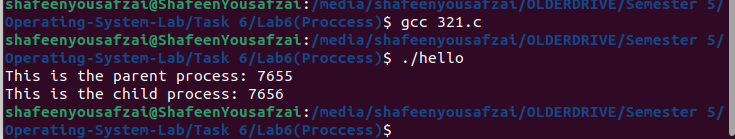
\includegraphics[width=\textwidth]{Screenshot from 2024-09-27 05-38-17.png}

\subsection{i<100}
  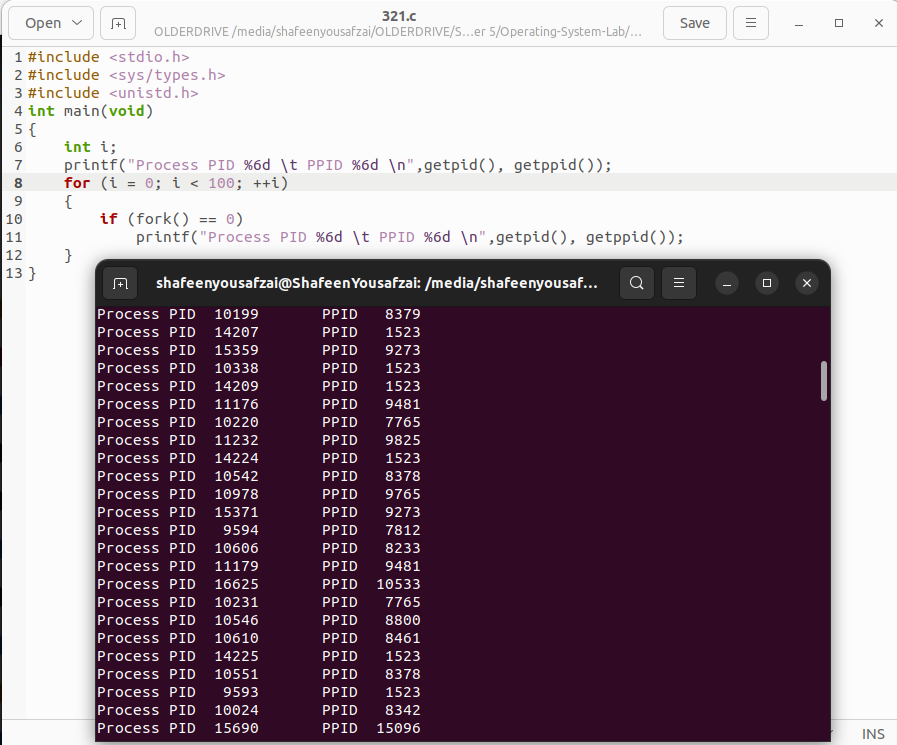
\includegraphics[width=\textwidth]{Screenshot from 2024-09-27 05-39-29.png}

\section{Fork Example}
\begin{verbatim}
#include <stdio.h>
#include <sys/types.h>
#include <unistd.h>

int main(void) {
    fork(); printf("He\n");
    fork(); printf("Ha\n");
    fork(); printf("Ho\n");
}
\end{verbatim}

\subsection{Q5 Answer}
Yes, a "Ho" can appear before a "He" due to the way processes execute concurrently.
  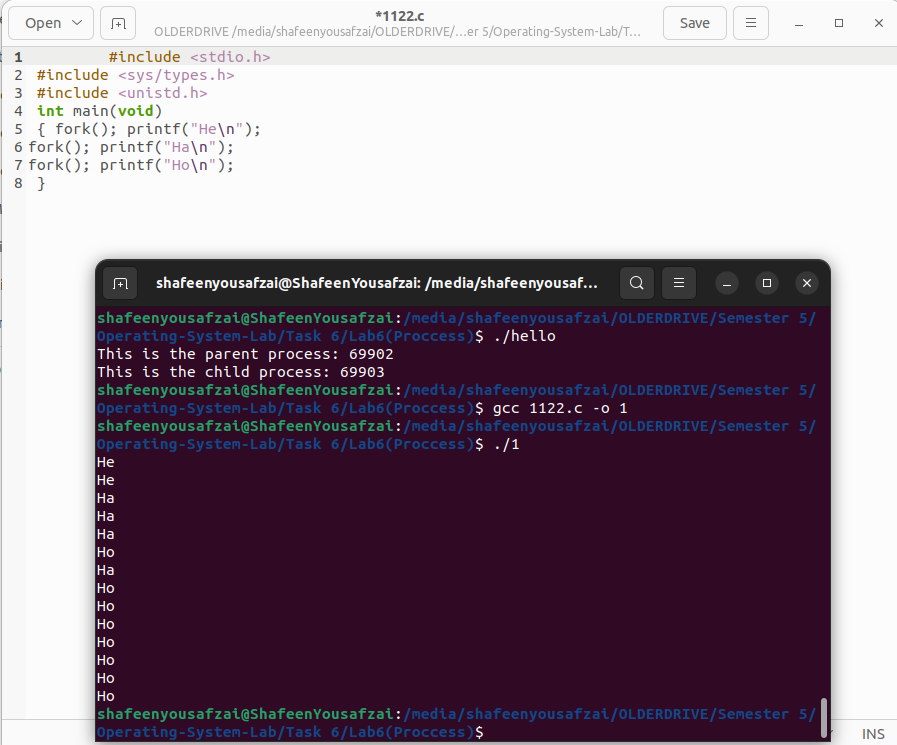
\includegraphics[width=\textwidth]{Screenshot from 2024-09-27 05-44-44.png}

\subsection{Q1 Answer}
We use p = fork() to distinguish between the parent (non-zero) and child (0) processes.

\subsection{Q2 Answer}
The printf() function is part of the <stdio.h> library.
\subsection{Q3 Answer}
"Job Done" is printed twice because both the parent and child processes execute the printf() after the fork().
\subsection{Q4 Answer}
The output will show the child PID in the parent process and 0 in the child process.
\section{3.2.1.1 Exercise 1}.
  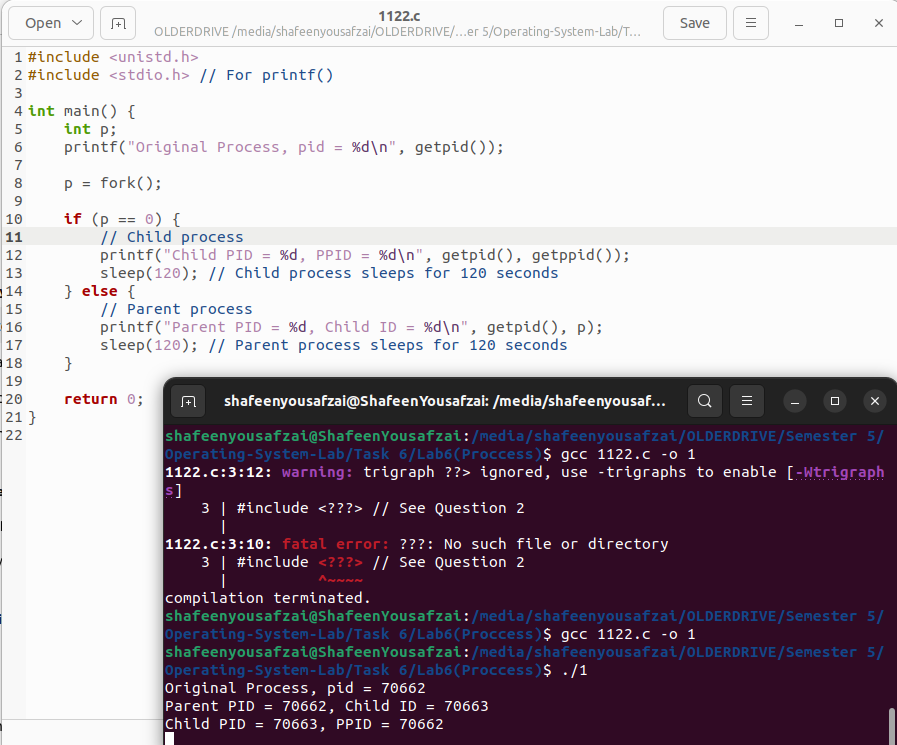
\includegraphics[width=\textwidth]{Screenshot from 2024-09-27 05-54-07.png}

\end{document}
